\documentclass[conference]{IEEEtran}
\IEEEoverridecommandlockouts

\usepackage[T1]{fontenc}
\usepackage[utf8]{inputenc}
\usepackage{cite}
\usepackage{amsmath,amssymb,amsfonts}
\usepackage{graphicx}
\usepackage{booktabs}
\usepackage{tikz}
\usetikzlibrary{positioning,arrows.meta,shapes.geometric,fit,backgrounds}
\usepackage{textcomp}
\usepackage{xcolor}
\usepackage{hyperref}

\def\BibTeX{{\rm B\kern-.05em{\sc i\kern-.025em b}\kern-.08em
    T\kern-.1667em\lower.7ex\hbox{E}\kern-.125emX}}

\begin{document}

% =====================================================================
% TODO (fill in before submission): your name, department, college/
% university, city, country, and email address below.
% =====================================================================
\title{Automated Fish Disease Diagnosis Using Hybrid AI:\\
A CNN--Vision Transformer Approach with Integrated Water Quality Monitoring}

\author{
\IEEEauthorblockN{Your Name}
\IEEEauthorblockA{
Department of Computer Science and Engineering\\
Your College Name, Your University\\
City, Country\\
your.email@example.com}
}

\maketitle

\begin{abstract}
Fish diseases are a major cause of yield loss in freshwater aquaculture, and manual visual diagnosis is slow, subjective, and depends on expert knowledge that small-scale farmers often lack. This paper presents SmartFish, an end-to-end web-based system for automated fish disease diagnosis. The core classifier is a hybrid deep learning architecture that fuses EfficientNet-B4 convolutional features with Vision Transformer (ViT-B/16) global features through multi-head cross-attention. Before classification, a classical computer-vision stage (Otsu thresholding and contour analysis) localizes the fish within the frame, and a lightweight ImageNet-pretrained gate rejects images that are not plausibly a fish. The classifier is trained on nine disease categories curated by merging two public Kaggle datasets, and is evaluated on a held-out test set of 780 images, achieving 97.18\% overall accuracy, a macro-averaged F1-score of 0.76, and a macro ROC-AUC of 0.969. We show that the comparatively low macro F1 is driven entirely by two severely underrepresented classes (5 and 2 test images respectively) rather than by the architecture, since the weighted F1 across all classes is 0.9675. The system also produces a best-effort ``affected region'' visualization from the classifier's own Vision Transformer attention weights, and is deployed as a FastAPI backend with a React frontend that additionally provides treatment/prevention guidance, diagnosis history, and a water-quality monitoring panel. We report the system's real, measured performance and its current limitations candidly, including the gap between the RT-DETRv2-based detector originally targeted and the classical-CV localization stage that was actually deployed due to the absence of bounding-box-annotated training data.
\end{abstract}

\begin{IEEEkeywords}
fish disease diagnosis, aquaculture, hybrid deep learning, EfficientNet, Vision Transformer, cross-attention fusion, water quality monitoring
\end{IEEEkeywords}

\section{Introduction}

Aquaculture is one of the fastest-growing sectors of global food production, and freshwater fish farming in particular is a major source of income for small and medium-scale farmers. Bacterial, fungal, viral, and parasitic diseases spread quickly in the confined, high-density conditions typical of farmed ponds and tanks, and early detection is the single most effective way to limit losses. In practice, however, diagnosis is usually done by visual inspection, either by the farmer or by a veterinary/extension worker who may not be available on short notice. This creates a real gap between when a disease becomes visible on a fish's body and when it is correctly identified and treated.

Deep learning-based image classification offers a way to close this gap: a farmer can photograph an affected fish and receive an immediate, consistent prediction rather than waiting for expert access. Convolutional neural networks (CNNs) have already been applied to fish disease and species classification with encouraging results \cite{dash2024,ergun2025}, and more recent work combines CNNs with additional techniques -- including explainability methods -- to make predictions more trustworthy \cite{utku2026}. Separately, Vision Transformers (ViTs) \cite{vit2021}, built on the self-attention mechanism \cite{attention2017}, have shown that global, long-range image context can complement the local texture features that CNNs excel at, and hybrid CNN--Transformer fusion has been shown to outperform either family alone in other fine-grained medical imaging tasks \cite{jayaraman2025}.

This paper describes SmartFish, a system that combines these ideas into a single deployed pipeline for freshwater fish disease diagnosis, rather than a classifier evaluated in isolation. The original design, matching a project poster titled ``Automated Fish Disease Diagnosis Using Hybrid AI,'' targeted an 11-class taxonomy with an RT-DETRv2 \cite{rtdetr2023} detection stage feeding a hybrid EfficientNet-B4/ViT-B16 classifier. During development we found that no public, usably-sized dataset provides bounding-box annotations for fish disease images -- only classification-style, pre-cropped images are available -- so a real detector could not be trained. We report this gap explicitly rather than silently substituting a different technique and describing it as the original design. The contributions of this paper are:

\begin{enumerate}
\item A hybrid EfficientNet-B4 + ViT-B/16 classifier, fused via multi-head cross-attention, trained on nine real disease classes curated by merging two public Kaggle datasets, with a fully reported, unmodified test-set evaluation (97.18\% accuracy, macro F1 0.76).
\item A lightweight fish-vs-non-fish gate built from an off-the-shelf ImageNet classifier's fish-related class probabilities, so the system can decline to diagnose an image that is not a fish instead of forcing it into one of the trained classes.
\item An attention-based ``affected region'' visualization derived directly from the classifier's own ViT branch, requiring no additional lesion-level annotation, together with an honest account of its limits as a saliency signal rather than a segmentation.
\item A complete, deployed full-stack system (FastAPI backend, React frontend) that pairs the classifier with treatment/prevention guidance, diagnosis history, and a water-quality monitoring panel, evaluated end-to-end rather than as a classifier alone.
\item A transparent discussion of where the deployed system falls short of the originally proposed design -- the substituted detection stage, and the two classes with too little data for the model to learn -- rather than a claim of matching an 11-class, fully-detected pipeline that was not actually achieved.
\end{enumerate}

The rest of this paper is organized as follows. Section II reviews related work in fish disease classification, hybrid CNN--Transformer architectures, and aquaculture monitoring. Section III describes the dataset, the localization and gating stages, the hybrid classifier, and the deployed system architecture. Section IV reports quantitative results, including per-class metrics, and discusses the two low-data classes and the qualitative behavior of the localization and explainability stages. Section V concludes and outlines future work.

\section{Related Work}

\subsection{Fish disease and species classification}
CNN-based classifiers have been applied directly to fish disease images. Dash et al.\ \cite{dash2024} fine-tuned a ResNet-50-based customized CNN for joint fish type and disease classification. Utku et al.\ \cite{utku2026} proposed a hybrid deep learning model for fish disease detection combined with explainable AI techniques to make predictions more interpretable to end users, a goal shared by the attention-based visualization used in this work. For the related task of fish species (rather than disease) identification, Ergün \cite{ergun2025} showed that a Swin Transformer backbone fine-tuned via transfer learning outperforms purely convolutional baselines, supporting the use of transformer-based global features for fine-grained fish image analysis in general.

\subsection{CNN, Vision Transformer, and hybrid fusion architectures}
EfficientNet \cite{efficientnet2019} introduced compound scaling of depth, width, and resolution to obtain strong accuracy-to-compute ratios, and remains a common transfer-learning backbone. The Vision Transformer \cite{vit2021} showed that a pure self-attention architecture \cite{attention2017}, applied to fixed-size image patches, can match or exceed CNNs when enough pretraining data is available. Because CNNs and ViTs capture complementary inductive biases -- local texture versus global context -- several recent works fuse the two rather than choosing one. Jayaraman et al.\ \cite{jayaraman2025} fused CNN and ViT features with cross-attention for brain tumor classification and reported gains over either backbone alone; the fusion mechanism used in this paper (projecting both branches to a shared dimension and fusing with multi-head cross-attention) follows the same principle, applied here to fish disease imagery instead of medical MRI scans.

\subsection{Detection stage}
RT-DETR \cite{rtdetr2023} introduced an end-to-end, NMS-free real-time detection transformer that outperforms YOLO-family detectors at comparable speed, and its successor RT-DETRv2 was the detector originally targeted for the fish-localization stage of this project. Training such a detector requires bounding-box-annotated data; the public fish disease datasets used in this work are classification-only (single fish, already cropped), so this project substitutes a classical computer-vision localization stage (Section~III-B) and reports this substitution explicitly rather than presenting classical CV results as if they came from a trained detector.

\subsection{Aquaculture water quality monitoring}
Water quality (pH, dissolved oxygen, temperature, ammonia) is tightly linked to both fish health and disease susceptibility. Mohd Jais et al.\ \cite{mohdjais2024} demonstrated a low-cost IoT multi-sensor system for real-time water quality monitoring in aquaculture tanks. The water-quality module in this paper is designed around the same parameters and the same intended use case, but -- unlike \cite{mohdjais2024} -- is currently simulated in software rather than backed by physical sensor hardware; Section~III-G discusses how the API is structured so that real sensors could be substituted without changing the frontend.

\section{Proposed Methodology}

\subsection{Dataset curation}
The poster's target taxonomy specifies 11 disease categories. No single public dataset covers all 11 with a usable number of images per class, so this project merges two Kaggle datasets: \emph{Freshwater Fish Disease Aquaculture in South Asia} \cite{kaggle-subirbiswas19}, which contributes Bacterial Aeromoniasis, Bacterial Gill Disease, Bacterial Red Disease, Fungal Saprolegniasis, Parasitic Disease, Viral White Tail Disease, and Healthy Fish ($\sim$350 images/class), and \emph{Fresh Water Fish Disease Dataset} \cite{kaggle-utpolkantidas}, a much smaller dataset from which Epizootic Ulcerative Syndrome (mapped to \emph{Ulcer\_Disease}) and \emph{Tail\_And\_Fin\_Rot} images are drawn (6--31 images per class before splitting). A physical-injury category (\emph{Broken Antennae and Rostrum}) present in the second dataset is not a disease under the poster's taxonomy and was deliberately excluded. This merge covers 9 of the poster's 11 target classes; \emph{Ich (White Spot Disease)} and \emph{Dropsy} have no usable public dataset at the time of writing and are not included as live predictions.

All images are resized to $224\times224$. Training-time augmentation consists of horizontal flipping, rotation, color jitter, and Gaussian noise/blur applied on-the-fly, together with CutMix applied to approximately 30\% of training batches. The data is split 70/15/15 (train/validation/test) at the image level with a fixed random seed; the source datasets provide no per-fish or per-farm identifier, so true subject-level separation between splits is not possible with this data. Table~\ref{tab:dataset} reports the resulting per-class image counts.

\begin{table}[htbp]
\caption{Per-class image counts after the 70/15/15 split}
\label{tab:dataset}
\centering
\begin{tabular}{lrrr}
\toprule
\textbf{Class} & \textbf{Train} & \textbf{Val} & \textbf{Test} \\
\midrule
Bacterial\_Aeromoniasis   & 344 & 102 & 105 \\
Bacterial\_Gill\_Disease  & 377 & 113 & 116 \\
Bacterial\_Red\_Disease   & 379 & 109 & 114 \\
Fungal\_Saprolegniasis    & 355 & 105 & 107 \\
Parasitic\_Disease        & 364 & 105 & 111 \\
Viral\_White\_Tail\_Disease & 346 & 103 & 100 \\
Healthy                   & 393 & 115 & 120 \\
Ulcer\_Disease            &  18 &   3 &   5 \\
Tail\_And\_Fin\_Rot       &   6 &   1 &   2 \\
\midrule
\textbf{Total}            & \textbf{2582} & \textbf{756} & \textbf{780} \\
\bottomrule
\end{tabular}
\end{table}

The last two rows make the central limitation of the dataset explicit: \emph{Ulcer\_Disease} and \emph{Tail\_And\_Fin\_Rot} have one to two orders of magnitude fewer images than the other seven classes, purely as a consequence of what is available in public data. Section~IV quantifies the effect this has on measured performance.

\subsection{Fish localization}
The original design used an RT-DETRv2 detector to localize the fish before cropping. Since no bounding-box-annotated dataset was available, this stage is instead implemented with classical computer vision: the input is converted to grayscale, blurred, and binarized with Otsu's thresholding; external contours are extracted, and contours covering at least 5\% of the frame area are unioned into a single bounding box, padded by 8\% on each side. A known failure mode of Otsu-based segmentation is that a close-up photo with no true background (e.g.\ a frame filled entirely by the fish) still gets bisected into two regions by the algorithm; naively keeping only the larger region then crops out part of the fish. This is detected heuristically: if the resulting box spans the full width or height of the frame edge-to-edge while covering a middling 25--85\% of the frame area, the stage falls back to using the full, uncropped frame instead of trusting the bisection. This localization stage is a stand-in for a trained detector, not a learned model, and is described as such throughout this paper.

\subsection{Fish presence gate}
Because the 9-class model has no explicit ``not a fish'' output, it will otherwise confidently force-fit any input -- including a photo of a person or an object -- into one of its trained classes. To avoid this, a pretrained MobileNetV3-Small ImageNet classifier is run on the (already localized) crop, and the summed softmax probability mass over sixteen fish/fish-like ImageNet classes (tench, goldfish, shark and ray species, eel, salmon, and related classes) is used as a coarse ``fish-likeness'' score. Images scoring below a threshold of 0.05 are rejected before the disease classifier runs. The threshold is set low deliberately: aquaculture species such as tilapia or catfish are not literally among ImageNet's 1000 classes, so even a genuine fish disease photo may only score moderately: the gate is tuned to catch clearly-not-a-fish input, not to be a strict fish-species validator.

\subsection{Hybrid classification architecture}
The disease classifier fuses two pretrained backbones:

\begin{itemize}
\item An \textbf{EfficientNet-B4} \cite{efficientnet2019} branch, used with its classification head removed and global pooling disabled, producing a spatial feature map that is adaptively average-pooled and projected (linear $\rightarrow$ ReLU $\rightarrow$ dropout) to a 512-dimensional vector.
\item A \textbf{ViT-B/16} \cite{vit2021} branch, used with its classification head removed, whose pooled output is projected through an identical linear $\rightarrow$ ReLU $\rightarrow$ dropout block to the same 512-dimensional space.
\end{itemize}

The two 512-dimensional tokens are stacked into a length-2 sequence and passed through an 8-head \texttt{MultiheadAttention} cross-attention layer \cite{attention2017}, allowing each branch's representation to attend to the other before fusion. The two attended tokens are concatenated (1024-dimensional) and passed through a fully connected classification head (1024 $\rightarrow$ 256 $\rightarrow$ 9) with ReLU and dropout ($p=0.3$). Figure~\ref{fig:architecture} summarizes the full inference pipeline, from input image to final prediction and UI response.

\begin{figure*}[t]
\centering
\resizebox{\textwidth}{!}{%
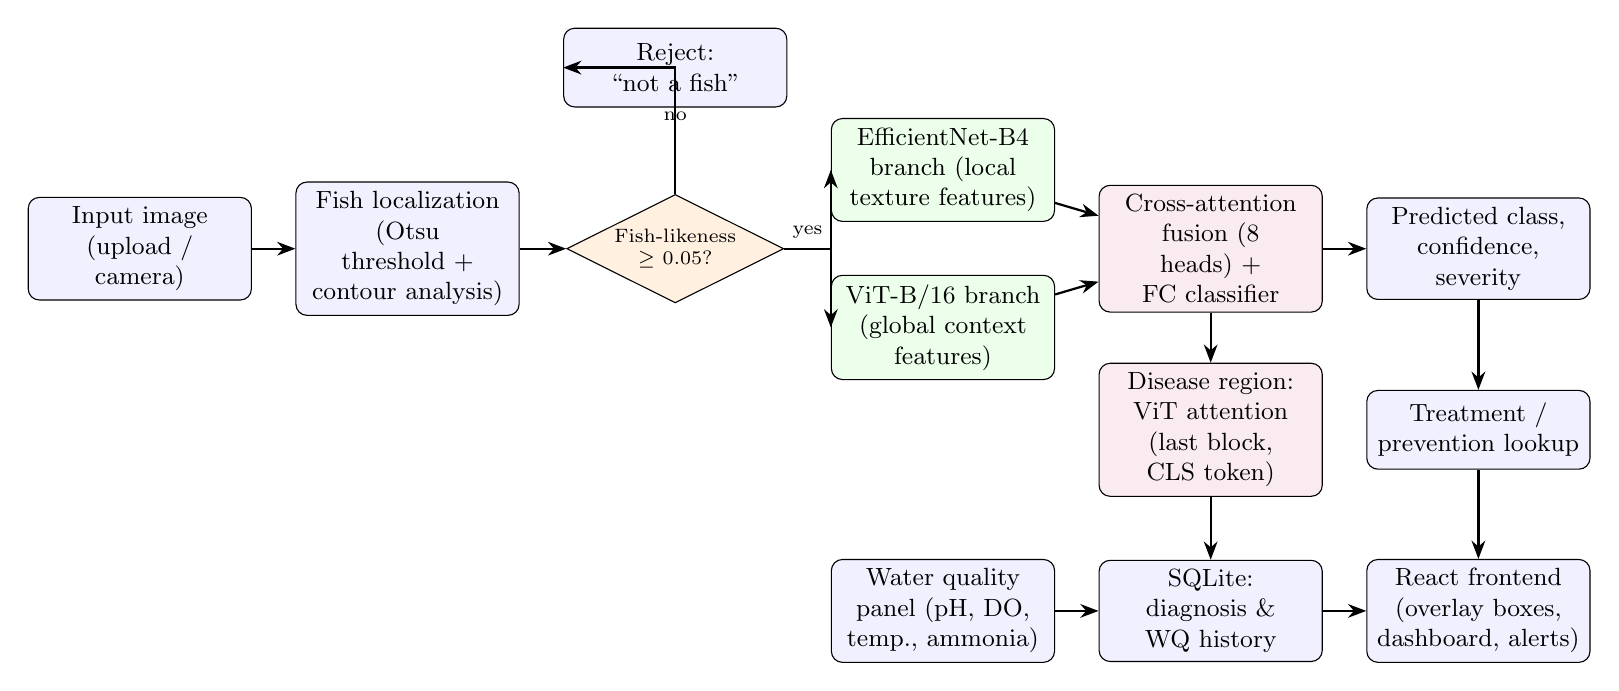
\begin{tikzpicture}[
  block/.style={rectangle, draw, rounded corners, fill=blue!6, align=center, minimum height=10mm, minimum width=27mm, text width=26mm, font=\small},
  decision/.style={diamond, draw, fill=orange!12, align=center, aspect=2.0, font=\scriptsize, inner sep=1pt},
  branch/.style={rectangle, draw, rounded corners, fill=green!8, align=center, minimum height=9mm, minimum width=27mm, text width=26mm, font=\small},
  smallblock/.style={rectangle, draw, rounded corners, fill=purple!8, align=center, minimum height=9mm, minimum width=27mm, text width=26mm, font=\small},
  arrow/.style={-Stealth, thick}
]
  % Explicit grid coordinates (cm) so nothing overlaps: columns at
  % x=0,3.4,6.8,10.2,13.6,17.0 ; rows at y=2.3 (reject), 0 (main flow),
  % -2.3 (secondary outputs), -4.6 (storage / UI).
  \node[block]    (input)  at (0,0)      {Input image\\(upload / camera)};
  \node[block]    (loc)    at (3.4,0)    {Fish localization\\(Otsu threshold +\\contour analysis)};
  \node[decision] (gate)   at (6.8,0)    {Fish-likeness\\$\geq$ 0.05?};
  \node[block]    (reject) at (6.8,2.3)  {Reject:\\``not a fish''};

  \node[branch]   (cnn)    at (10.2,1.0) {EfficientNet-B4\\branch (local\\texture features)};
  \node[branch]   (vit)    at (10.2,-1.0){ViT-B/16 branch\\(global context\\features)};
  \node[smallblock] (fusion) at (13.6,0) {Cross-attention\\fusion (8 heads) +\\FC classifier};
  \node[block]    (pred)   at (17.0,0)   {Predicted class,\\confidence,\\severity};

  \node[smallblock] (region) at (13.6,-2.3) {Disease region:\\ViT attention\\(last block, CLS token)};
  \node[block]    (rec)    at (17.0,-2.3) {Treatment /\\prevention lookup};

  \node[block]    (wq) at (10.2,-4.6) {Water quality\\panel (pH, DO,\\temp., ammonia)};
  \node[block]    (db) at (13.6,-4.6) {SQLite:\\diagnosis \&\\WQ history};
  \node[block]    (ui) at (17.0,-4.6) {React frontend\\(overlay boxes,\\dashboard, alerts)};

  \draw[arrow] (input) -- (loc);
  \draw[arrow] (loc) -- (gate);
  \draw[arrow] (gate.north) |- node[near start, above, font=\scriptsize]{no} (reject.west);
  \draw[arrow] (gate.east) -| node[near start, above, font=\scriptsize]{yes} (cnn.west);
  \draw[arrow] (gate.east) -| (vit.west);
  \draw[arrow] (cnn) -- (fusion);
  \draw[arrow] (vit) -- (fusion);
  \draw[arrow] (fusion) -- (pred);
  \draw[arrow] (fusion) -- (region);
  \draw[arrow] (pred) -- (rec);
  \draw[arrow] (region) -- (db);
  \draw[arrow] (rec) -- (ui);
  \draw[arrow] (wq) -- (db);
  \draw[arrow] (db) -- (ui);
\end{tikzpicture}%
}
\caption{End-to-end SmartFish pipeline: classical-CV fish localization, an ImageNet-based fish presence gate, the EfficientNet-B4/ViT-B16 cross-attention classifier, ViT-attention-based disease region visualization, and the surrounding full-stack system (treatment lookup, water-quality panel, SQLite history, React frontend).}
\label{fig:architecture}
\end{figure*}

\subsection{Training configuration}
The model is trained with the AdamW optimizer (learning rate $1\times10^{-4}$, weight decay $1\times10^{-4}$), cross-entropy loss, and a \texttt{ReduceLROnPlateau} schedule, with batch size 32. Training was run for 10 epochs on a free-tier Google Colab T4 GPU, with the checkpoint selected by best validation loss; the selected checkpoint (epoch 9 of 10, zero-indexed) reached a validation accuracy of 97.62\% and a validation loss of 0.0897. The epoch budget was set deliberately low to fit within free-tier Colab session limits; the training script supports early stopping with a patience of 10 epochs and up to 100 epochs for longer runs on dedicated hardware.

\subsection{Disease region attention visualization}
To give the user some visual indication of what the model responded to, the system exposes the ViT branch's own attention rather than training a separate explainability model. timm's default \texttt{Attention} implementation uses a fused scaled-dot-product-attention kernel that never materializes attention weights, so the last ViT block's forward method is replaced with a numerically identical implementation that additionally caches its post-softmax attention. At inference time, the CLS token's attention to all image patches in the last block is averaged over attention heads, reshaped to its native $14\times14$ grid, and upsampled to the crop's resolution with Gaussian smoothing applied both before and after resizing. Because last-layer ViT attention is well known to spread across several disjoint regions rather than concentrating on one, thresholding at a fixed fraction of the maximum value would span nearly the whole image; instead, an 80th-percentile threshold is applied and only the single largest connected component (by contour area) is kept, offset back into the original image's coordinate space.

This visualization is explicitly \emph{not} a pixel-precise lesion segmentation: no lesion-level (pixel-wise disease-region) annotations exist for this dataset, so the visualization cannot be trained or validated against ground truth, only sanity-checked mechanically (the returned box always lies within the image bounds and degrades gracefully to the full crop when no clear attention peak exists). During development, manual inspection on real photographs showed the highlighted region does not always align tightly with the visibly diseased area of the fish; we report this as a genuine limitation of relying on classification-only attention as a localization signal, not as a solved component of the system.

\subsection{System architecture and deployment}
The backend is implemented in FastAPI with five endpoints: \texttt{/health}, \texttt{/detect-fish} (localization + gate only, used for the frontend's fast first-step preview), \texttt{/predict} (full diagnosis), \texttt{/history}, and \texttt{/water-quality} (GET/POST). Diagnosis records and water-quality readings are persisted with SQLAlchemy to a local SQLite database. The frontend is a React (Vite) single-page application with five pages (Home, Detection, Water Quality, Dashboard, Alerts); the Detection page supports both file upload and live camera capture, and draws the fish-localization box and the disease-attention box as two independently colored overlays on an HTML canvas positioned over the preview image. The water-quality panel currently simulates pH, temperature, dissolved oxygen, and ammonia readings with rule-based status/alert logic, but is deliberately built behind the same REST contract that a real sensor deployment such as \cite{mohdjais2024} would use, so that simulated readings could be replaced by real hardware without changing the frontend. For local network deployment, the frontend resolves its API base URL from \texttt{window.location.hostname} at runtime and the backend binds to \texttt{0.0.0.0}, allowing any device on the same network to reach a running instance without a code change or public hosting.

\section{Results and Discussion}

\subsection{Classification performance}
The classifier is evaluated once, on the untouched 780-image test split (Table~\ref{tab:dataset}), with no threshold or hyperparameter tuning performed against test-set results. Table~\ref{tab:results} reports precision, recall, and F1-score per class. Overall test accuracy is 97.18\%, with a macro-averaged precision of 0.757, macro recall of 0.763, macro F1 of 0.760, macro specificity of 0.996, and a macro (one-vs-rest) ROC-AUC of 0.969.

\begin{table}[htbp]
\caption{Per-class test-set performance ($n=780$)}
\label{tab:results}
\centering
\begin{tabular}{lrrrr}
\toprule
\textbf{Class} & \textbf{Prec.} & \textbf{Recall} & \textbf{F1} & \textbf{Supp.} \\
\midrule
Bacterial\_Aeromoniasis   & 1.000 & 0.981 & 0.990 & 105 \\
Bacterial\_Gill\_Disease  & 0.975 & 0.991 & 0.983 & 116 \\
Bacterial\_Red\_Disease   & 0.948 & 0.965 & 0.957 & 114 \\
Fungal\_Saprolegniasis    & 0.982 & 1.000 & 0.991 & 107 \\
Parasitic\_Disease        & 0.991 & 0.964 & 0.977 & 111 \\
Viral\_White\_Tail\_Disease & 0.980 & 0.970 & 0.975 & 100 \\
Healthy                   & 0.937 & 0.992 & 0.964 & 120 \\
Ulcer\_Disease            & 0.000 & 0.000 & 0.000 &   5 \\
Tail\_And\_Fin\_Rot       & 0.000 & 0.000 & 0.000 &   2 \\
\midrule
\textbf{Accuracy}         & \multicolumn{3}{r}{\textbf{0.9718}} & \textbf{780} \\
\textbf{Macro avg}        & 0.757 & 0.763 & 0.760 & 780 \\
\textbf{Weighted avg}     & 0.964 & 0.972 & 0.968 & 780 \\
\bottomrule
\end{tabular}
\end{table}

Figures~\ref{fig:cm} and \ref{fig:roc} show the confusion matrix and per-class ROC curves. Both confirm the same pattern visible in Table~\ref{tab:results}: the seven classes with adequate training data (346--393 training images) are classified with F1-scores between 0.957 and 0.991, and the confusion between them is concentrated almost entirely between the visually similar bacterial disease classes, as expected.

\begin{figure}[htbp]
\centering
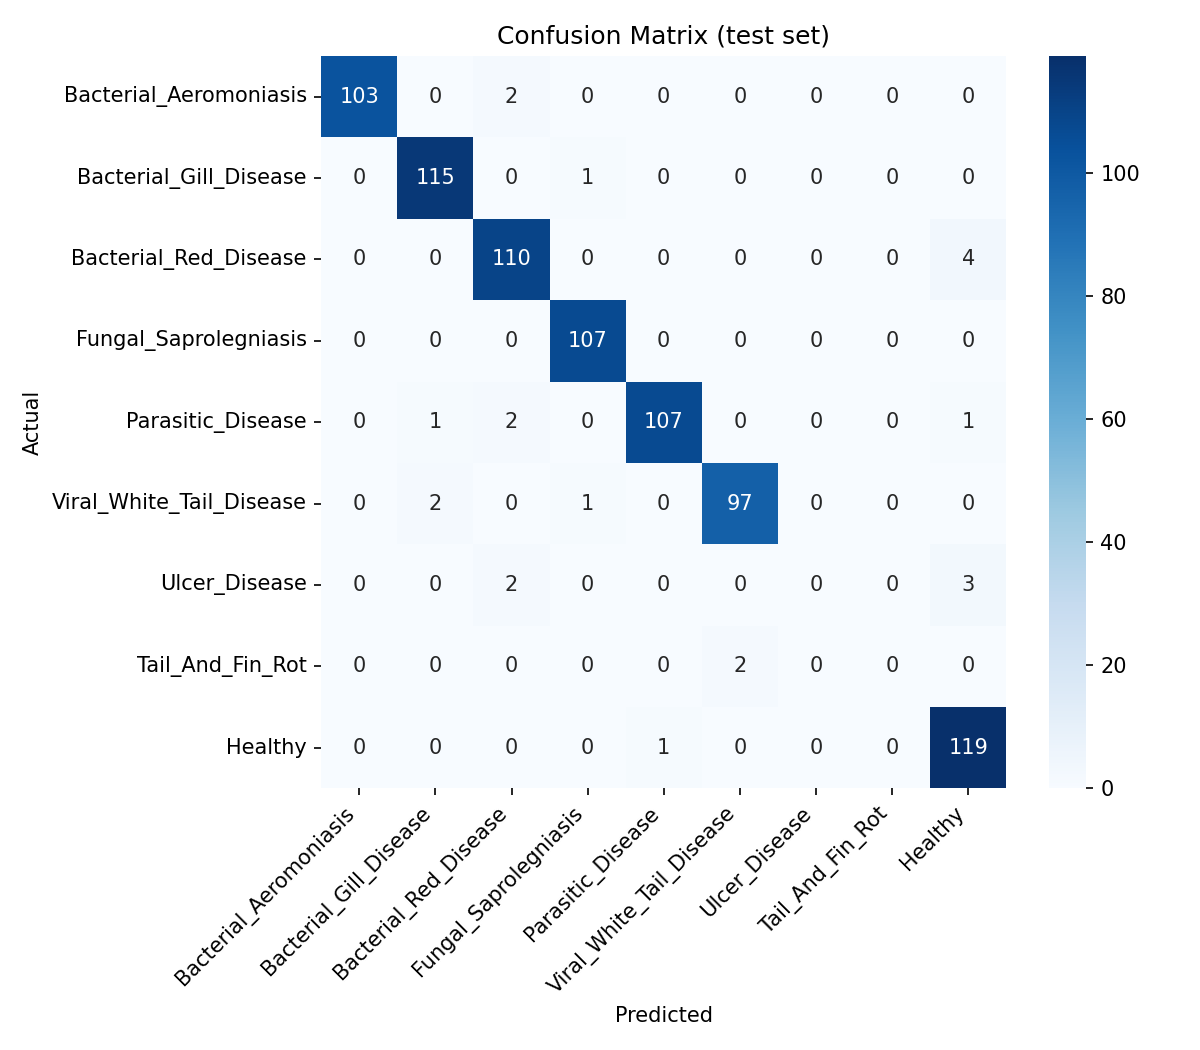
\includegraphics[width=\linewidth]{figures/confusion_matrix.png}
\caption{Confusion matrix on the held-out test set (780 images, 9 classes).}
\label{fig:cm}
\end{figure}

\begin{figure}[htbp]
\centering
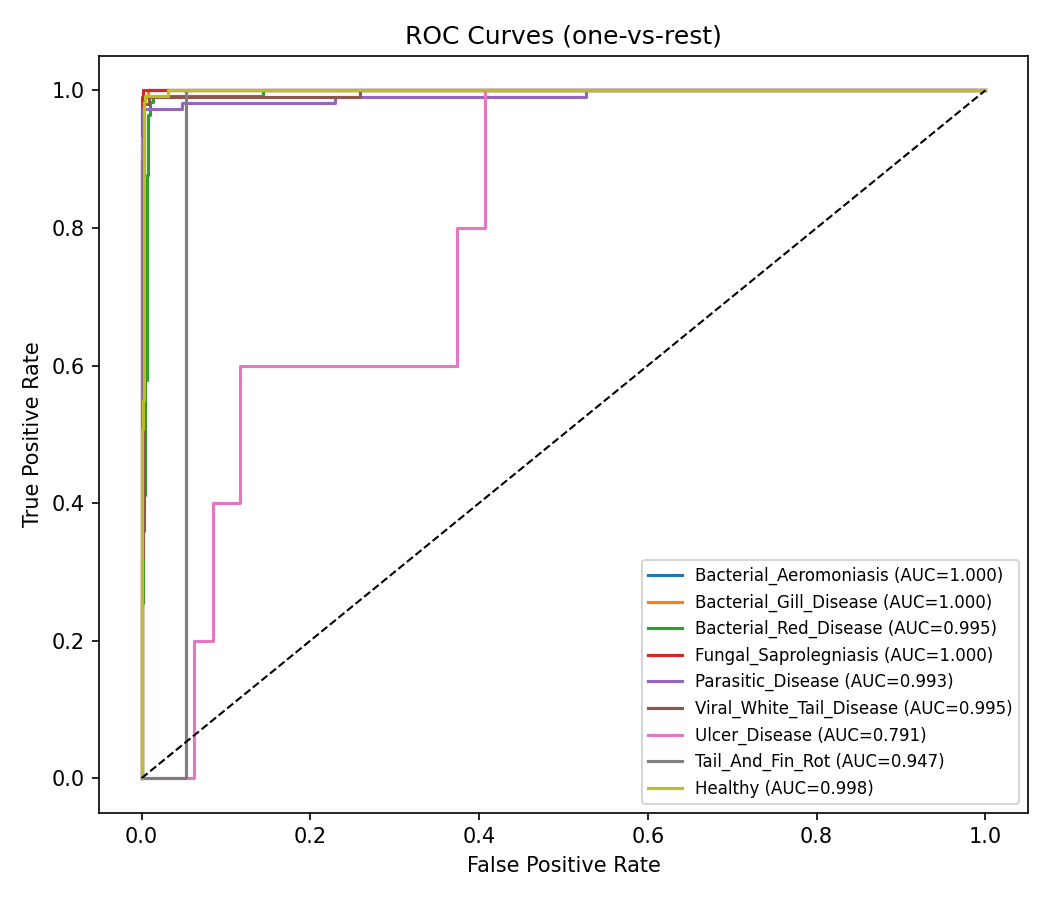
\includegraphics[width=\linewidth]{figures/roc_curves.png}
\caption{One-vs-rest ROC curves per class; macro-averaged AUC is 0.969.}
\label{fig:roc}
\end{figure}

\subsection{The effect of the two low-data classes}
\emph{Ulcer\_Disease} and \emph{Tail\_And\_Fin\_Rot} score 0.000 on precision, recall, and F1, despite perfect specificity (1.000): with only 18 and 6 training images respectively, the model never learns to predict either class, so it neither correctly identifies nor falsely predicts them on the test set. This is the entire explanation for the gap between the very high weighted-average F1 (0.968, which reflects that these two classes make up only 7 of 780 test images, under 1\%) and the much lower macro-average F1 (0.760, which weights all nine classes equally regardless of support). We report macro metrics rather than omitting them or reporting only accuracy, because a macro average is the honest way to surface a class-imbalance problem that a single accuracy number hides. This is a data-volume limitation, not an architecture limitation: the same model architecture reaches F1 $>$ 0.95 on every class that has a comparable amount of training data to the others.

\subsection{Qualitative evaluation of localization and the disease-attention overlay}
Neither the fish-localization stage nor the disease-attention visualization has ground-truth bounding boxes or lesion masks available in the dataset, so both were evaluated qualitatively during development rather than with a quantitative metric such as IoU. The localization stage's edge-span heuristic (Section~III-B) was validated against a set of synthetic test cases (a fish silhouette on a plain background, a close-up filling the full frame, and a frame split by strong internal shading) and correctly avoided cropping into the fish in all three. On real photographs, the fish-localization box reliably contains the whole fish. The disease-attention overlay is qualitatively less reliable: on real disease photographs tested during development, the highlighted region sometimes falls on a plausible part of the fish and sometimes does not track the visibly diseased area. We attribute this to the combination of a coarse $14\times14$ attention grid, the lack of any lesion-level supervision during training, and the CLS token's attention being a global-context signal rather than a class-conditional saliency map by construction. We present it to the user as a best-effort visual aid, not a diagnostic-grade localization, and consider improving it -- most plausibly via a small amount of lesion-level annotation -- a priority for future work rather than a solved problem.

\subsection{Limitations}
We summarize the honest limitations of the current system: (1) only 9 of the poster's 11 target disease classes have any usable public data, and 2 of those 9 have too little data to be learned reliably; (2) the fish-localization stage is classical computer vision, not the trained RT-DETRv2 detector originally targeted, because no bounding-box-annotated dataset exists for this task; (3) the disease-attention visualization is a best-effort saliency signal from an off-the-shelf attention mechanism, not a validated lesion segmentation; (4) the train/validation/test split is at the image level, not the subject/farm level, because the source datasets provide no such identifier; and (5) the water-quality panel is currently simulated rather than backed by physical sensors.

\section{Conclusion and Future Work}
This paper presented SmartFish, a deployed hybrid EfficientNet-B4/ViT-B16 fish disease diagnosis system that reaches 97.18\% test accuracy on a 9-class, 780-image held-out test set, with a macro F1 of 0.76 that we show is attributable to two data-starved classes rather than to the model. Beyond the classifier, the system provides a fish-presence gate, an attention-based disease-region visualization, and a full-stack deployment with treatment guidance, diagnosis history, and a water-quality panel. We reported the gap between this system and the originally targeted 11-class, RT-DETRv2-detected design explicitly, rather than presenting a substituted classical-CV localization stage as if it were a trained detector.

Future work follows directly from the limitations in Section~IV-D: collecting or annotating more images for \emph{Ulcer\_Disease} and \emph{Tail\_And\_Fin\_Rot}, and for the two entirely missing classes (\emph{Ich} and \emph{Dropsy}); annotating a bounding-box dataset (e.g.\ via Roboflow) so a real RT-DETRv2 detector can replace the classical-CV localization stage; collecting a small lesion-level annotated subset to properly train and evaluate the disease-region visualization rather than relying on unsupervised attention; and integrating physical pH/dissolved-oxygen/temperature/ammonia sensors behind the existing water-quality API, following the low-cost sensor design demonstrated in \cite{mohdjais2024}.

\bibliographystyle{IEEEtran}
\bibliography{references}

\end{document}
